%% ----------------------------------------------------------------------------
% CVG SA/MA thesis template
%
% Created 03/08/2024 by Tobias Fischer
%% ----------------------------------------------------------------------------
\documentclass[pdftex,11pt,openright,headsepline]{book}
\usepackage[margin=1in,headheight=13.6pt]{geometry}

\usepackage{paralist}		% List environment
\usepackage{color}		% For colored text
\usepackage{times}
\usepackage{amsfonts}		% Additional math fonts
\usepackage{amsmath}		% Math symbols
\usepackage{latexsym}
\usepackage{graphicx}		% For including images
% \usepackage{listings}		% If listings are needed
\usepackage{macros}		% Our own definitions
% \usepackage{wrapfig}		% To wrap images
% \usepackage{algorithmic}	% Nice algorithm environment
% \usepackage{algorithm}
\usepackage{fancyhdr}		% Produce the nice header
%\usepackage{fullpage} % Use the full page


\usepackage[colorlinks=true, linkcolor=blue, citecolor=blue, urlcolor=black]{hyperref}

% Change the appearance of the header. Here \MakeUppercase is hard-coded, so renewing this command allows to elegantly change the header appearance.
\renewcommand{\MakeUppercase}{\scshape}

% Set the headings' appearance in the ``fancy'' pagestyle
\fancyhead{}
\fancyhead[RO, LE]{\leftmark}
\fancyfoot{}
\fancyfoot[RO, LE]{\thepage}

% The first pages shall be empty, even no page numbering 
\usepackage{setspace}
\setstretch{1.2}


\begin{document}
\pagestyle{empty} % even no page number

\fancypagestyle{plain}{
  \renewcommand{\headrulewidth}{0.0pt}
  \fancyfoot{}
  \fancyhead{}
}

% Title page, modify accordingly 
%% ----------------------------------------------------------------------------
% CVG SA/MA thesis template
%
% Created 03/08/2024 by Tobias Fischer
%% ----------------------------------------------------------------------------

\begin{titlepage}

\thispagestyle{empty}

\fancypagestyle{empty}{
\lhead{
\includegraphics[height=1.5cm]{images/ethlogo_black}}
\renewcommand{\headrulewidth}{0.0pt}
\rhead{\vspace*{-0.2cm}
\includegraphics[height=1.4cm]{images/cvgLogo.pdf}}
\fancyfoot{}
}



\vspace*{2cm}
\begin{center}
\Huge{\textbf{MSc. Thesis Title
}\\}
\LARGE{\textbf{Subtitle}\\[1cm]}
\vspace{5pt}
\large{Master's Thesis\\[0.8cm]}
\LARGE{Amalie Kjaer\\}
\normalsize{Department of Computer Science D-INFK}
\end{center}

\vfill
\begin{center}
\begin{tabular}{ll}
\Large{\textbf Advisors:} & \Large{Dr.~Zuria Bauer, Dr.~Mihai Dusmanu}\\
\Large{\textbf Supervisor:} & \Large{Prof.~Dr.~Marc Pollefeys}\\
			    & \small{Computer Vision and Geometry Group}\\
			    & \small{Department of Computer Science D-INFK}\\
\end{tabular}
\end{center}

\begin{center}
\today\\
\end{center}


\end{titlepage}


\cleardoublepage

%% ----------------------------------------------------------------------------
% CVG SA/MA thesis template
%
% Created 03/08/2024 by Tobias Fischer
%% ----------------------------------------------------------------------------

\newpage
\vspace{3cm}

\chapter*{Abstract}
\noindent The abstract gives a concise overview of the work you have done. The reader should be able to decide whether the work that has been done is interesting for him by reading the abstract. Provide a brief account of the following questions:

\begin{itemize}
 \item What is the problem you worked on? (Introduction)
 \item What are the shortcomings of existing solutions? (Technical Gap)
 \item How did you tackle the problem? (Method)
 \item What were your results and findings? (Experiments)
 \item Why are your findings significant? (Conclusion)
\end{itemize}

\noindent The abstract should approximately cover half of a page, and does generally not contain citations.




% Input here any acknowledgements
%% ----------------------------------------------------------------------------
% CVG SA/MA thesis template
%
% Created 03/08/2024 by Tobias Fischer
%% ----------------------------------------------------------------------------


\newpage

\chapter*{Acknowledgements}


\cleardoublepage
\newpage

% % Chapter-pages etc. use the ``plain'' pagestyle - since we don't want to have a heading at all at chapter-pages, redefine plain accordingly. Don't forget the page number. 
\fancypagestyle{plain}{
  \renewcommand{\headrulewidth}{0.0pt}
  \fancyfoot{}
  \fancyfoot[RO, LE]{\thepage}
  \fancyhead{}
}

\pagestyle{fancy}
\pagenumbering{Roman}

% Insert table of contents
\tableofcontents

% % Insert list of figures
% \listoffigures
% \cleardoublepage

% % Insert list of tables
% \listoftables
% \cleardoublepage

% \newpage

\pagenumbering{arabic}

%% ----------------------------------------------------------------------------
% Actual text comes here - defer it to other files and use \input{bla.tex}, ..
%% ----------------------------------------------------------------------------
%% ----------------------------------------------------------------------------
% CVG SA/MA thesis template
%
% Created 03/08/2024 by Tobias Fischer
%% ----------------------------------------------------------------------------


\chapter{Introduction}
Give an introduction to the topic you have worked on:

\begin{itemize}
 \item \textit{What is the rationale for your work?} Motivate the problem, \eg with a general description of the problem setting, narrowing down to the particular problem you have been working on in your thesis. Allow the reader to understand the problem setting. 
 \item \textit{What is the technical gap in existing work?} Briefly outline how this problem has been tackled before, and what the shortcomings of the existing solutions are.
 \item \textit{What is your work doing to fix it?} Given the above background, state briefly the focus of the work. 
\end{itemize}

Motivation
The problem
Challenges
Objectives / Goals
Contributions
Methods
Existing work
Structure of the thesis
Main results
%% ----------------------------------------------------------------------------
% CVG SA/MA thesis template
%
% Created 03/08/2024 by Tobias Fischer
%% ----------------------------------------------------------------------------

\newpage
\chapter{Related Work}

The related work section has the following purposes: 

\begin{itemize}
 \item \textit{Is the overview concise?} Give an overview of the most relevant work to the needed extent. Make sure the reader can understand your work without referring to other literature.
 \item \textit{Does the compilation of work help to define the ``niche'' you are working in?} Another purpose of this section is to lay the groundwork for showing that you did significant work. The selection and presentation of the related work should enable you to name the implications, differences, and similarities sufficiently in the discussion section.
\end{itemize}

description of task
\section{Visual Question Answering Task (indoor + other)}

VQA vs 3D-QA

indoor is a subtask but it is interesting because we can include some 3D element to it
- also this lays the foundation for answering harder questions later on, which cannot be answered simply with 2D methods: eg. about distances and paths, which would be interesting for navigation tasks.
\begin{itemize}
    \item Task description
    \item Expected inputs / outputs
    \item Question ontology
    \item Classical methods (non-SG), strenghts and limitations
    \item Scene Graph methods (Graph Question Answering), strengths and limitations (most of these for indoor scenes say they use graphs but they never utilise edge info)
\end{itemize}

description of data
\section{Scene Graphs}
\begin{itemize}
    \item Scene graph formal definition + advantages
    \item Scene graph generation methods
    \item Graph neural networks
    \item Applications and limitations
\end{itemize}


description of the "building blocks" used to create the model
\section{Image-text pretrained models}

\section{Transformer encoder / decoders}
GNN can be formulated as a 

\section{Existing datasets}


\newpage
\chapter{Datasets}
\textbf{ScanNet}
The ScanNet dataset consists of 1,513 annotated point clouds of 3D-indoor environments, generated from 2,492,518 annotated RGB-D frames. The dataset includes a wide range of spaces such as offices, apartments, bathrooms, classrooms, libraries, and more. It spans both small spaces (e.g., bathrooms, closets) and large spaces (e.g., studio apartments, classrooms). The dataset is annotated with instance-level and semantic-level (NYU40) labels.

Note: In most existing SSG methods, the scene must first be segmented. However, to get a more accurate scene graph dataset, we opt to use the segmentation already provided by ScanNet. we use oracle segmentation (we assume perfect segmentation is available).

Note: we remove scenes with segmentation errors (some segmented objects do not appear in any of the images -- specifically scenes 180, 279, 305, 530, 597)
[Plot scene / label distribution]

\noindent
\textbf{ScanQA}
The ScanQA dataset consists of xxx questions about the ScanNet scenes.
We prepare x different question datasets to experiment on: 1) easy 2) hard 3) complete/mixed 4) constant scenes
[Plot question / answer distribution]

Limitations: although ScanQA is designed for 3D-VQA, most of the questions do not require 3D information to answer (ie could be answered with 2D images only). This is because the questions are generated from the 2D images of the scenes (check this fact?). Ie. no questions about distances, paths, dimensions, geometry, etc.

Removed multiple answer questions (lower performance on this)

\newpage
\chapter{Method}

%-----------------------------
% METHODS INTRODUCTION
% Remember to include:
% - What problem are you solving formally (inputs, outputs, assumptions)
% - How are you solving this problem
%-----------------------------
This project addresses the task of Visual Question Answering within 3D indoor environments (3D-VQA). 3D-VQA consists in answering open-vocabulary, free-form questions about an environment. For example, given segmented RGB-D images of a hallway and the question "Where did I put my keys?", the 3D-VQA model should be able to locate the keys in the scene and output an accurate response to the question, such as "On top of the drawer at position ($x, y, z$)".

The two main challenges of the 3D-VQA task are 1) to create a rich scene representation, often starting from RGB-D frames and 2) to combine this scene representation with a text query to produce an accurate output answer. The 3D-VQA task therefore requires merging different data modalities in a multimodal model to condition the output answer on the given question-scene input pairs.

While current research often claims to utilize scene graphs as scene representations, it solely relies on node information, and does not utilize edge information in the VQA model. This means that current methods do not leverage the full potential of scene graphs. Furthermore, existing VQA models often rely solely on pre-trained language-vision models, such as CLIP, to bring the question and scene representation into the same embedding space, lacking a learning mechanism.

To mitigate these limitations, we propose:
\begin{enumerate}
    \item a dataset of scene graphs for the ScanNet dataset (ScanNet-SG), paired with questions about the graphs from the ScanQA dataset. This is, to our knowledge, the first dataset of question-scene graph pairs for 3D indoor environments.
    \item an end-to-end 3D-VQA classification model which combines graph and text modalities to answer questions about the scene.
\end{enumerate}

We emphasize that our proposed VQA model is a classificaton model, rather than a generation model. This means that the model does not aim to output free-form answers, but rather to solve the task of selecting the object in the scene which is most relevant to the question posed. For example, the question "What color is the chair by the desk" should return the instance of "chair", rather than the answer "the chair is black". In other words, the proposed model returns the object in the scene which is most relevant to the question (where someone should look to answer the question), rather than the actual answer to the question. This classification task is easier to evaluate and interpret than the generation task, and a good starting point for evaluating the model's ability to understand question-scene pairs. Furthermore, solving the classification task first ensures that we can train a model that does not rely on textual priors to answer questions, since the model must focus on instance accuracy rather than semantic accuracy. This forces the model to learn to understand the scene and the question. Our model can be easily extended to a generation model by adding a decoder component to the model.

The following sections detail the scene graph generation method used to obtain the ScanNet-SG dataset, as well as the proposed 3D-VQA classification models.






\section{Scene Graph Generation}

[Add that we use scannet labels to embed rather than nyu40 because its more descriptive / larger more precise vocabulary than nyu40]
[specify that for clip we are using the huggingface implementation]

[Add figure here] (each step summarized)

We aim produce semantically meaningful graph representations of the ScanNet indoor scenes. 
[best possible preserve scene structure / translate all the important pointcloud information into a scene graph]
To achieve this, we let graph nodes represent segmented objects in the scene, and graph edges represent proximity, such that nearby nodes are connected by an edge. We note that there is no such "ground truth" representation, since scene graph generation requires some design choices. More specifically, to construct a graph representation $G = (V, A, E)$, the following components must be defined:

\begin{enumerate}
    \item \textbf{Node features, $V \in \mathbb{R}^{n \times D_V}$: } the graph contains $n$ nodes with $D$-dimensional embedding, which encodes information about the object it represents.
    \item \textbf{Adjacency, $A \in \mathbb{R}^{n \times n}$:} the graph edges are defined in an $n \times n$ adjacency matrix, which encodes information about which nodes are connected. Node connectivity can represent any type of node similarity, such as proximity, visual similarity, semantic similarity, functional similarity, etc.
    \item \textbf{Edge features, $E \in \mathbb{R}^{|A| \times D_E} $: } Optionally, edge embeddings $E$ (which represent edge features), can also be defined. An example of edge labels could be the description of the relation between nodes, such as "next to", "inside", "above", "same color", "same function", ...
\end{enumerate}

The following sections detail the scene graph generation method used in this paper.

\subsection{Node features}
We initialize the node embeddings with CLIP-embedded images of the object of interest. However, as each object may appear in many RGB-D frames under different views, we must select which views to embed, and how to combine these into a single node embedding.

\bigskip
\noindent
\textbf{View Selection}
Given the high frame rate of the image capture, we discard every other RGB-D image in each scene to speed up the data processing. The best views for each object are then selected by calculating a "view score": firstly, we use the 3D pointcloud segmentation to obtain the 3D-coordinates of a tight, axis-aligned bounding box for each object in the scene. The coordinates of the bounding box corners are then projected into each RGB-frame. Projecting the bounding box corners into each frame allows us to determine whether the object is fully visible in the frame, or only partly visible. Then, for each object in the scene, we rank views according the following score $s$:

\begin{equation*}
    s = \frac{n}{w \times h} \times \frac{b}{8},
\end{equation*}

where $n$ is the number of pixels occupied by the object in the frame, $w$ and $h$ are the width and height of the frame and $b$ is the number of bounding box corners visible in the frame (out of 8 possible corners). The first term in this score is the "size term", which represents how much space the object takes up in the frame (the larger the object, the better). The second term is the "visibility term", which represents how much of the total object is visible in the frame (the entire object is better than only part of the object). Hence a score close to $1$ signals a close-up view of a fully visible object, whereas a score close to $0$ signals either a distant view, or a partial view, or both. This method therefore attributes low scores to zoomed-in partial views and distant views, and large scores to large, complete views of an object. We note that weights could be added to both the "size" and "visibility" components of the score to weigh their relative importance.

+ Using the 3D bb corner projections assumes that the entire object is visible in the frame dataset (if only half an object was photographed, the bb will obviously be smaller than GT since the 3D segmentation is obtained from the 2D segmentation)

\bigskip
\noindent
\textbf{Cropping}
For each object, we then select the top-k views and crop these around the object of interest. Three different cropping methods were tested: 1) a tight, non-square crop around the object with all pixels not belonging to the object blacked out, 2) a tight crop, non-square around the object with no further changes, 3) a square crop around the object, resized to $224 \times 224$.

Figure XX illustrates these cropping methods:

\bigskip
\noindent
\textbf{Embedding}
Since CLIP was trained on square images and can only embed square images, for cropping methods 1) and 2) the standard CLIP pre-processing was used: resizing the shortest edge to 224 and randomly selecting a $224 \times 224$ crop within the image. Then we CLIP embed the top-k views and aggregate them with a score-weighted average, yielding a single CLIP-embedding for each object that captures view variability and gives a more rich embedding to the object node.

Section xx quantitatively compares the weighted CLIP embeddings obtained using each of the cropping methods described above.

+ justify why we use CLIP (brings text + images into the same embedding space, hopefully in semantically meaningful, should be a good initialization for a model).

\subsection{Adjacency}
Adjacency matrix is the component of the graph which allows us to encode/transfer 3D information of the scene into the graph. The adjacency matrix in the provided dataset was chosen to represent spatial proximity of nodes. Therefore, the shortest distance between each object should be calculated, and edges should exist only between objects with a distance less than some predetermined heuristic threshold. Several methods were explored to calculate or approximate the shortest distance between objects.
Figure XX illustrates these methods.

\bigskip
\noindent
\textbf{Naive approach: Pointcloud-based shortest distance}
First, a naive approach was implemented: the shortest distance between two objects was calculated by computing the distance between all 3D points of 2 object pointclouds. Although this is the most accurate measure of shortest distance, it is too computationally expensive and also very sensitive to outliers. We therefore decided to approximate the shortest distance between two objects rather than accurately computing it.

\bigskip
\noindent
\textbf{Approximation approach: Axis-aligned bounding box shortest distance}
To approximate the shortest distance between two pointclouds, we obtain the axis-aligned bounding box for each object from the 3D scene segmentation. The shortest distance between two axis-aligned boundign boxes can then be calculated as:


A threshold of 0.2 was selected heuristically. We note that this measure is not very precise. Results can be changed by varying the threshold.

The adjacency matrix is symmetrized to ensure bidirectional relationships between nodes. Additionally, self-loops are added to represent self-relationships.

\subsection{Edge features}
We compare two learning-based approaches to annotate/predict the edge label of the edges determined above.

\bigskip
\noindent
\textbf{Random Forest}

\bigskip
\noindent
\textbf{MLP}






\newpage
\section{VQA Models}
%-----------------------------
% VQA MODEL METHODS
%-----------------------------

Figure XX illustrates the general 3D-VQA classification method. VQA models take as inputs a question and a scene graph (generated as described above), and outputs the most relevant object in the scene to the question. Regardless of architecture, any VQA model must have the following components: 1) a scene encoder, 2) a question encoder, 3) object selection head, which combine scene and question encodings to select the output object.

We explore solutions for each of these components, and compare the performance of three distinct families of model architectures: a baseline model (no learning), a GNN-only (learning only for scene encoding) model, and a transformer-based model (learning for scene encoding, question encoding and selection head). Some of the components are shared across models, this helps us identify which components of the final proposed model are actually helpful.

The following sections detail the architecture and design choices of each model.

\subsection{Baseline Model}
The baseline model is used to establish a lower bound on the performance of the VQA task. The baseline model is illustrated in Figure XXX. It does not require any learning, and relies solely on the pre-computed CLIP embeddings of the objects in the scene and the question. The model consists of the following components:

\textbf{Scene Encoder:} The scenes are encoded as the set of its ScanNet-SG scene graph nodes (without edges, obtained as described in section XXX).

\textbf{Question Encoder:} The question encoding is the sentence-level CLIP embedding of the question.

\textbf{Object Selection Head:} The model computes the cosine similarity between the question embedding and the node embeddings of the scene graph. The node with the highest similarity is selected as the output object.

While this baseline model is a simple and common approach to the VQA task [ref], it has some important limitations. Firslty, the scene encoder encurs a large information loss: by discarding edges, it does not encode any 3D or structural information about the scene. It therefore does not capture the overall room layout, and lacks contextual awareness. This implies that objects with similar appearance may have indifferentiable encodings, regardless of their context and neighbouring objects, and that the overall scene encoding does not change if even if objects are moved around. For example, the baseline model may not be able to differentiate between a chair in the middle of the room and a chair in the corner of the room, as the scene representation would be the same. This means that while semantic accuracy might be high, instance accuracy is expected to be low. Furthermore, the model has no learning mechanism, meaning that the scene representation cannot adapt to new questions.

\subsection{GNN-only Model}
To address these limitations, we explore the GNN-only model, which uses a graph neural network to learn better node embeddings. The model is illustrated in Figure XXX. The model consists of the following components:

\textbf{Scene Encoder:} The ScanNet-SG scene graphs are passed through a dimension-preserving GNN. The GNN updates node embeddings iteratively by aggregating information from neighbouring nodes. This ensures each node becomes aware of its context.

- What type of GNN architecture? How many layers? How many hidden units? What activation function? What aggregation function? What loss function?

\textbf{Question Encoder:} Same as the baseline model.

\textbf{Object Selection Head:} Same as the baseline model.

The GNN-only model is expected to perform better than the baseline model, as structural information is added to the scene encoding. This model should therefore better differentiate between objects with similar appearance but different context. Furthermore, the scene encoder is learned, meaning that the model can learn to adapt scene encodings to better match the question encoding. In other words, the model can learn to align the question and scene embeddings in a learned way, rather than a fixed way as in the baseline model. However, the GNN-only model still has some limitations. Firstly, the model is still limited by the question encoding and object selection, which are not learned. This means that the model may struggle  with questions that are not well-aligned with the learned scene graph.

\subsection{Transformer-based Models}

The transformer-based model incorporates learning for the question encoding and object selection head. It is illustrated in Figure XXX. The idea was to create a model with more degrees of freedom than the GNN-only model: instead of trying to align the fixed question embeddings and learned scene embeddings using cosine similarity, the model learns to predict a  score for each object instance in the scene based on the learned scene and question embeddings. High score indicates high relevance to the question.

The model is composed of four main components: 1) a question encoder, 2) a scene graph encoder, 3) a cross-attention mechanism, and 4) a classifier.

The question encoder is a transformer-based model which encodes the question into a fixed-size vector. The scene graph encoder is a graph neural network which encodes the scene graph into a fixed-size vector. The classifier is a multi-layer perceptron which takes the question and scene graph embeddings as input and outputs the most relevant object in the scene to the question.

How many layers? How many hidden units? What activation function? What aggregation function? What edge update function? What loss function?

\subsection{Loss function}

\textbf{Cross-entropy loss}
\textbf{Multi-object Cross-entropy loss}
\textbf{Focal loss}
%% ----------------------------------------------------------------------------
% CVG SA/MA thesis template
%
% Created 03/08/2024 by Tobias Fischer
%% ----------------------------------------------------------------------------
\newpage
\chapter{Experiments}

[We prepare x different question datasets to experiment on: 1) easy 2) hard 3) complete/mixed 4) constant scenes]

In this section, we detail experimental methods and results for the generation of the ScanSG dataset and the proposed ScanSG-Transformer model.

\section{Scene Graph Generation}

[Note: we remove scenes with segmentation errors (some segmented objects do not appear in any of the images -- specifically scenes 180, 279, 305, 530, 597)]

In order to train a successful 3D-VQA model, we must ensure that its input data, namely generated scene graphs and questions, are of high quality. This section empirically evaluates the impact of different design choices on the quality of the generated scene graphs. We evaluate the design choices for scene graph nodes and edges separately, and choose the best performing parameters for the proposed scene graph dataset. For scene graph nodes, we evaluate the effects of different cropping methods, k-values, and visibility scores on the quality of the node embeddings. For scene graph edges, we evaluate the impact of different threshold values on the quality of the edges in the scene graphs.

All experiments in this section are performed on a smaller subset of the dataset, consisting of 71 scenes, with a total of 2467 objects across scenes. This subset is also used for testing in section XXX.

\subsection{Node Construction}
We evaluate the impact of different cropping methods, k-values and visibility scores on the quality of the generated node CLIP-embeddings. The following paragraphs detail the methods and parameters considered for each of these design choices.

\bigskip \noindent
\textbf{Cropping method:}
We compare the impact of the following cropping methods on node embedding quality (illustrated in Figure XXX):
\begin{enumerate}
    \item A tight, rectangular crop around the object with all background pixels masked out. With this method, the object is centered in the image, and the background is removed. However, CLIP was trained on square images with no background removal. To adapt rectangular crops to CLIP, we use the resizing method described in the original CLIP paper [XXX]: the crop is resized to $224$ in its minimum dimension, and then randomly cropped to a $224 \times 224$ square.
    
    \item A tight, rectangular crop around the object with no further changes. With this method, the object is centered in the image. However, the background is not removed, meaning other surrounding objects could contribute to the embedding, and the image is not square. The rectangular crops are resized as in the original CLIP paper [XXX].
    
    \item A square crop centred around the object, resized to $224 \times 224$. With this method, the crop is square and correctly sized, and no further processing is needed. However, the background is not removed and the non-tight crop means other surrounding objects might contribute to the node embedding.
    
    \item A tight, rectangular crop, resized to $224 \times 224$. With this method, the crop is tight around the object (fewer surrounding objects included in the crop). However, the resized crops distort the image, and CLIP was not trained on distorted images.
\end{enumerate}

\begin{figure}[h!]
    \centering
    \begin{minipage}[b]{0.1\textwidth}
        \centering
        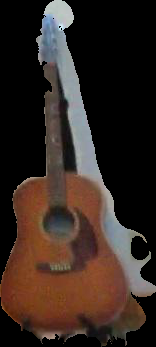
\includegraphics[width=\textwidth]{images/cropping_method_0.png}
        \caption{Caption 1}
    \end{minipage}
    \hspace{1em} % Adjust this to control the horizontal space between images
    \begin{minipage}[b]{0.1\textwidth}
        \centering
        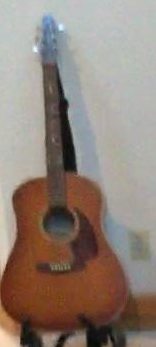
\includegraphics[width=\textwidth]{images/cropping_method_1.png}
        \caption{Caption 2}
    \end{minipage}
    \vspace{0em} % Adjust this to control the vertical space between rows
    \begin{minipage}[b]{0.1\textwidth}
        \centering
        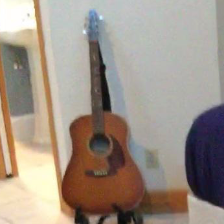
\includegraphics[width=\textwidth]{images/cropping_method_2.png}
        \caption{Caption 3}
    \end{minipage}
    \hspace{1em} % Adjust this to control the horizontal space between images
    \begin{minipage}[b]{0.1\textwidth}
        \centering
        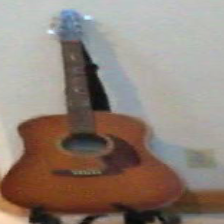
\includegraphics[width=\textwidth]{images/cropping_method_3.png}
        \caption{Caption 4}
    \end{minipage}
    \caption{Overall figure caption}
\end{figure}

\bigskip \noindent
\textbf{k-value:}
We also evaluate the impact of different k-values on the quality of the scene graph nodes. The k-value determines how many images of the object will be considered when generating the scene graph node. A higher value of k could result in a more accurate representation of the object, but could also introduce noise or inconsistencies as different views may have different different embeddings. We not that increasing the k-value highly increases the computational cost. It is therefore important to find the optimal k-value that balances these trade-offs. In this analysis we consider the following k-values: $k=1$, $k=3$, and $k=10$.

\bigskip \noindent
\textbf{Visibility score:}
\begin{enumerate}
    \item $s_1 = \frac{n}{w \times h} \times \frac{b}{8}$
    \item $s_2 = w_p \frac{n}{w \times h} + w_c \frac{b}{8}$ with $w_p = 1$, $w_c = 1$
    \item $s_2$ with $w_p = 100$, $w_c = 1$
    \item $s_2$ with $w_p = 1$, $w_c = 100$
\end{enumerate}

To evaluate the comparative quality of these cropping methods and k-values, we perform the following experiment: first, we generate scene graphs using each of the three cropping methods, with $k=1$, $k=3$ and $k=10$ respectively. We therefore have a total of 9 different scene graph node generation methods. Then, we CLIP-embed all the object labels in the scene, and calculate the similarity between the embeddings of the object crops and the embeddings of the object labels. For each object, we select the label with the highest similarity, and compare it to the ground truth label. We calculate the accuracy of the scene graph nodes for each of the 9 methods, and choose the best performing method for the final model.  Note that we only use semantic accuracy (since there is no context-awareness mechanism or learning in this experiment) to evaluate the quality of the scene graph nodes. The semantic accuracy is the percentage of nodes that are embedded closest to their label in the CLIP embedding space. We repeat this experiment for each visibility score listed above, keeping the cropping method and k-value constant. Tables XX shows the results of this experiment.

\begin{table}[h!]
    \centering
    \caption{}
    \begin{tabular}{l|lll|}
    \cline{2-4}
                                                   & \multicolumn{3}{c|}{\textbf{k-value}} \\ \hline
    \multicolumn{1}{|c|}{\textbf{Cropping method}} & 1        & 3       & 10               \\ \hline
    \multicolumn{1}{|l|}{Tight masked crop}        & 49.5     & 50.1    & 52.1             \\
    \multicolumn{1}{|l|}{Tight crop}               & 57.6     & 58.9    & 60.3             \\
    \multicolumn{1}{|l|}{Square crop}              & 57.1     & 58.3    & \textbf{62.2}    \\
    \multicolumn{1}{|l|}{Tight resized crop}       & 56.2     & 57.4    & 60.2             \\ \hline
    \end{tabular}
\end{table}
\begin{table}[h!]
    \centering
    \caption{}
    \begin{tabular}{|c|c|}
    \hline
    \textbf{Visibility Score} & \textbf{Accuracy} \\ \hline
    s1                       & 62.2               \\ \hline
    s2                        & 78.2                  \\ \hline
    s3                        &                   \\ \hline
    s4                        &                   \\ \hline
    \end{tabular}
\end{table}

\bigskip
\noindent
\textbf{Results and Interpretation}

Table XX shows some examples of inaccurate node embeddings. The table shows the crop of the object, the ground truth label, and the label with the highest similarity to the object crop. These inaccuracies are most often caused by other objects appearing in the object of interest's crop for the following reasons:
\begin{itemize}
    \item they occlude the object of interest (see floor example)
    \item they are contained within the object of interest (see doorframe example)
    \item they are similar to the object of interest (see shelf example)
    \item the object of interest is rectangular so a square crop includes other objects (see guitar case example)
\end{itemize}

\begin{table}[h]
    \centering
    \caption{\textcolor{red}{add the GT and pred label under each image, show them all side by side.}}
    \begin{tabular}{|c|l|l|}
        \hline
        \textbf{Crop} & \textbf{Ground Truth Label} & \textbf{Most Similar Label} \\ \hline
        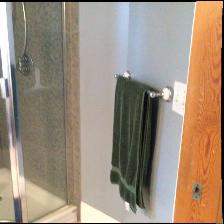
\includegraphics[width=1in]{images/wall.png} & Wall & Shower \\ \hline
        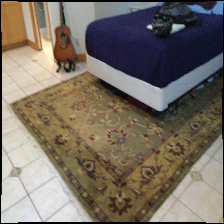
\includegraphics[width=1in]{images/floor.png} & Floor & Bed \\ \hline
        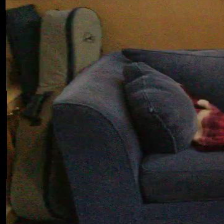
\includegraphics[width=1in]{images/guitar case.png} & Guitar Case & Couch \\ \hline
        
\includegraphics[width=1in]{images/doorframe.png} & Doorframe & Door \\ \hline
        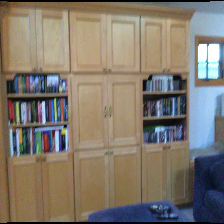
\includegraphics[width=1in]{images/shelf.png} & Shelf & Cabinet \\ \hline
    \end{tabular}
\end{table}

These examples highlight some inherent limitations of the CLIP method. However, we believe CLIP embeddings are still a good starting points as they offer a common embedding for the images in text, which is accurate in most cases.

\textcolor{red}{showcases some of the important clip limitations. we further discuss these limitations in Section XX (Discussion). }

The experiments also highlight the necessity of including some learning into the model, because the CLIP-embedding of the object is not very close to the CLIP-embedding of the object label. And this label task is easier than the question task, as shown in Figure XXX.


\subsection{Edge Construction}
Same model, same node embeddings (only change is the edges).

\begin{table}[h!]
    \centering
    \caption{accuracy (percent)}
    \begin{tabular}{|c|c|}
    \hline
    \multicolumn{1}{|l|}{\textbf{Threshold value (m)}} & \textbf{EM@1 (\%)} \\ \hline
    0.2                                                & \textbf{20.1}      \\ \hline
    0.5                                                & 14.6               \\ \hline
    0.8                                                & 9.8                \\ \hline
    Random edges                                       & 4.0                \\ \hline
    \end{tabular}
    \end{table}

Dense graphs perform better than sparse graphs. Cannot use no edges because then the scene structure is lost.
So these edges help the model learn.

We train GNN model on the scene graphs with different threshold values for the edges. We evaluate the performance of the model on the test set, and choose the best threshold value for the final sg dataset. We also compare the performance of the model with the best threshold value to the performance of the model with random edges. Table XXX shows the results of this experiment.

Simple GNN model -> show that chosen threshold is better than random edges.
Also show that edges can have a huge impact on the final answer --> must be chosen carefully.



\subsection{Edge Label Classification}

\subsection{Dataset Statistics}
(Add to appendix instead)
Average number of edges per graph, "impact window"? ...


%%%%%%%%%%%%%%%%%%%%%%%%%%%%%%%%%%%% VQA %%%%%%%%%%%%%%%%%%%%%%%%%%%%%%%%%%

\section{Visual Question Answering Model}

In this section, we assess the performance of each model described in section XXX on the generated ScanSG dataset. The evaluation metrics and hyperparameters common to all experiments are described below. The details specific to each experiment are described in the relevant sections, such that the results can be reproduced.

\textcolor{red}{
Our model introduces 2 new components compared to the traditional baseline: edge information + cross-attention. This section investigates the added benefit of each component in the context of the ScanSG + ScanQA dataset.}

\textcolor{red}{
Turns out cross attention definitely contributes to higher performance (the ScanSG-noGNN always outperforms the baseline). The GNN does not actually contribute, but this is most likely because it is not suited to this dataset. this dataset contains very little data which can actually take advantage of the gnn structure. In conclusion, this is the best we can do with the data we have. Need better Q dataset (maybe one that lists all possible answers!!), and maybe need to think of other ways to embed the nodes (such as owl?).
}

\subsection{GraphVQA}
\textcolor{red}{
what we tried, the results were random on the scenes tested.
the main issue was that this method relies on the "programs" but we had none for this method.
so this is also a sign that the model was overfit to their specific dataset.}

\subsection{Experimental Setup}

\bigskip
\noindent \textbf{Dataset}
The test/train split from the original ScanQA paper [XXX] is used. Multi-answer questions are removed such that each question has exactly one answer. Unless otherwise stated, the training set consits of $92\%$ of the dataset with 19,500 questions about 555 scenes. The test set consists of the remaining $8\%$ with 1,581 questions about 71 scenes. The scenes in the training and test set are kept separate, such that during testing, the model sees new questions about unseen scenes.

\bigskip
\noindent \textbf{Hyperparameters}
For the baseline model, no training is required, hence none of the following hyperparameters are relevant. For all other models, a batch size of $64$ was used for all experiments. The Adam optimizer was used with a learning rate tuned to each model. The loss function used was the cross-entropy loss, except if stated otherwise. The models were trained for $200$ epochs.

\bigskip
\noindent \textbf{Evaluation metrics}
We compare the performance of each model on the test set of the ScanSG dataset, and report the results in terms of best EM@1 (same as instance accuracy), EM@5 and EM@10 achieved. EM@K is the percentage of questions for which the correct answer is in the top-K predicted answers. We report three measures of EM@K to understand the performance at different levels of accuracy, and monitor these metrics during training to understand how the models learn. An increasing EM@10 score indicates that the model is learning to predict the correct answer with higher confidence, while an increasing EM@1 score indicates that the model is learning to predict the correct answer with higher accuracy. We also report the semantic accuracy, Sem-EM@1. The semantic accuracy indicates correct label prediction, regardless of predicted instance. A high discrepancy between EM@1 and Sem-EM@1 indicates that the model correctly identifies the answer label, but struggles to identify the correct instance of this label. Table XXX summarizes the results achieved by each model.

\bigskip
\noindent \textbf{Loss function}
The cross-entropy loss is used across all experiments, unless stated otherwise.

\subsection{Model Performance on ScanSG + ScanQA}

Table XX shows the performance of each model on the generated ScanSG+ScanQA dataset.

\begin{table}[h!]
    \centering
    \caption{Performance on the full ScanSG+ScanQA dataset, with node embeddings computed from the top-k image crops, as described in XX.}
    \begin{tabular}{|l|c|c|c|c|}
    \hline
    \textbf{Model}         & \textbf{EM@1} & \textbf{EM@5} & \textbf{EM@10} & \textbf{Sem-EM@1} \\ \hline
    Baseline               & 28.1 & 59.7 & 73.8 & 36.4  \\ \hline
    Baseline + GNN         & 12.3 & 38.8 & 54.3 & 18.9  \\ \hline
    ScanSG-GNN             & 25.3 & 64.2 & 81.2 & 33.5 \\ \hline
    ScanSG-noGNN           & \textbf{43.6} & \textbf{73.9} & \textbf{86.6} & \textbf{55.7} \\ \hline
    \end{tabular}
\end{table}

\bigskip \noindent
\textbf{Baseline}
Since the baseline model does not require any training, it is simply evaluated on the test set of the ScanSG dataset. The hyperparameters and loss function are irrelevant.

The baseline model does not utilize edge information (which encodes scene structure and 3D information), and thus does not have the ability to differentiate between instances of the same object class. This results in a higher semantic accuracy (Sem-EM@1) than instance accuracy (EM@1), as seen in Table XX.

Furthermore, since the baseline relies on static, pre-computed text and image embeddings, it cannot learn from the data. While this makes the baseline a highly generalisable model, it also means that the model performs poorly on samples where CLIP(question) has a dissimilar pre-computed embedding than CLIP(answer). Since CLIP was trained on descriptive captions rather than questions about the image, it is expected that question embeddings may not align with their associated answer.


\bigskip \noindent
\textbf{Baseline + GNN}
\textcolor{red}{Learning rate for Baseline + GNN:}

The Basline+GNN model adds a learning component to the Baseline model, in the form of a GCN which propagates node information to its neighbours, such that each node gains an awareness of its surroundings. This makes for a context-aware scene representation.

However, Table XX shows that this method performs worse than the simple baseline. This can be explained by the fact that the Baseline + GNN model computes the cosine similarity between a dynamic, learnable embedding (nodes) and a static, pre-computed embedding (question). This method incentivises the model to update node embeddings such that they better align with the questions they answer. However, as some questions have the same answer but very different embeddings, this creates conflicting training examples. Noisy data impedes model learning.

\textcolor{red}{+ maybe add a figure to illustrate this}

\textcolor{red}{+ also maybe not enough data that actually needs a gnn. pull these two conclusions together in the final conclusion}

\bigskip \noindent
\textbf{ScanSG-GNN}
The ScanSG-GNN model adds learnable, word-level text embeddings, and a cross-attention mechanism. The performance of this model is similar to that of the basline model, but with higher confidence (higher EM@5 and EM@10 scores than the baseline).

\bigskip \noindent
\textbf{ScanSG-noGNN}
This model is the ScanSG-GNN model stripped of the GNN. The difference between ScanSG-noGNN and the baseline is that there is word-level embedding and a cross-attention mechanism.

This model outperforms the ScanSG-GNN model. However, since it has been stripped of the GNN, it has no context awareness (two scenes with the same objects in different positions would have the same encoding), and should not be able to answer relational questions. This means that the model is not learning the scene structure but rather language priors.

This model performs the best, indicating that the cross-attention mechanism with the word-level embeddings work better than the cosine similarity of embeddings. This also indicates that the GNN does not benefit model performance.

\bigskip
\noindent
We note that all models display strong overfitting. \textcolor{red}{add proof in appendix.}
In the following section, we address the following questions, which arise from the experiment: 1) Can we regularize the ScanSG model to prevent overfitting? 2) Can the overfitting be explained by poor data quality? and 3) Why does the GNN component decrease accuracy?

\textcolor{red}{likely because the gnn is data hungry and there is not that much data that requires information propagation. the hard questions do but also they are likely too hard (even for human, they have many possible answers).}


\subsection{Addressing Overfitting}
The discrepancy between the train and test accuracy (and loss) suggests that the models suffer from overfitting. This is further illustrated in Figures XXX. While the train accuracy increases with increasing number of training epochs, the test accuracy initially increases, and starts to decrease after around 6 epochs. In Figure XXX, the train loss decreases with increasing number of epochs, whereas the test loss initially decreases, and then starts to increase around 6 epochs. This indicates that the model is overfitting to the training data, limiting its generalization to the test data.

% \begin{figure}[h!]
%     \centering
%     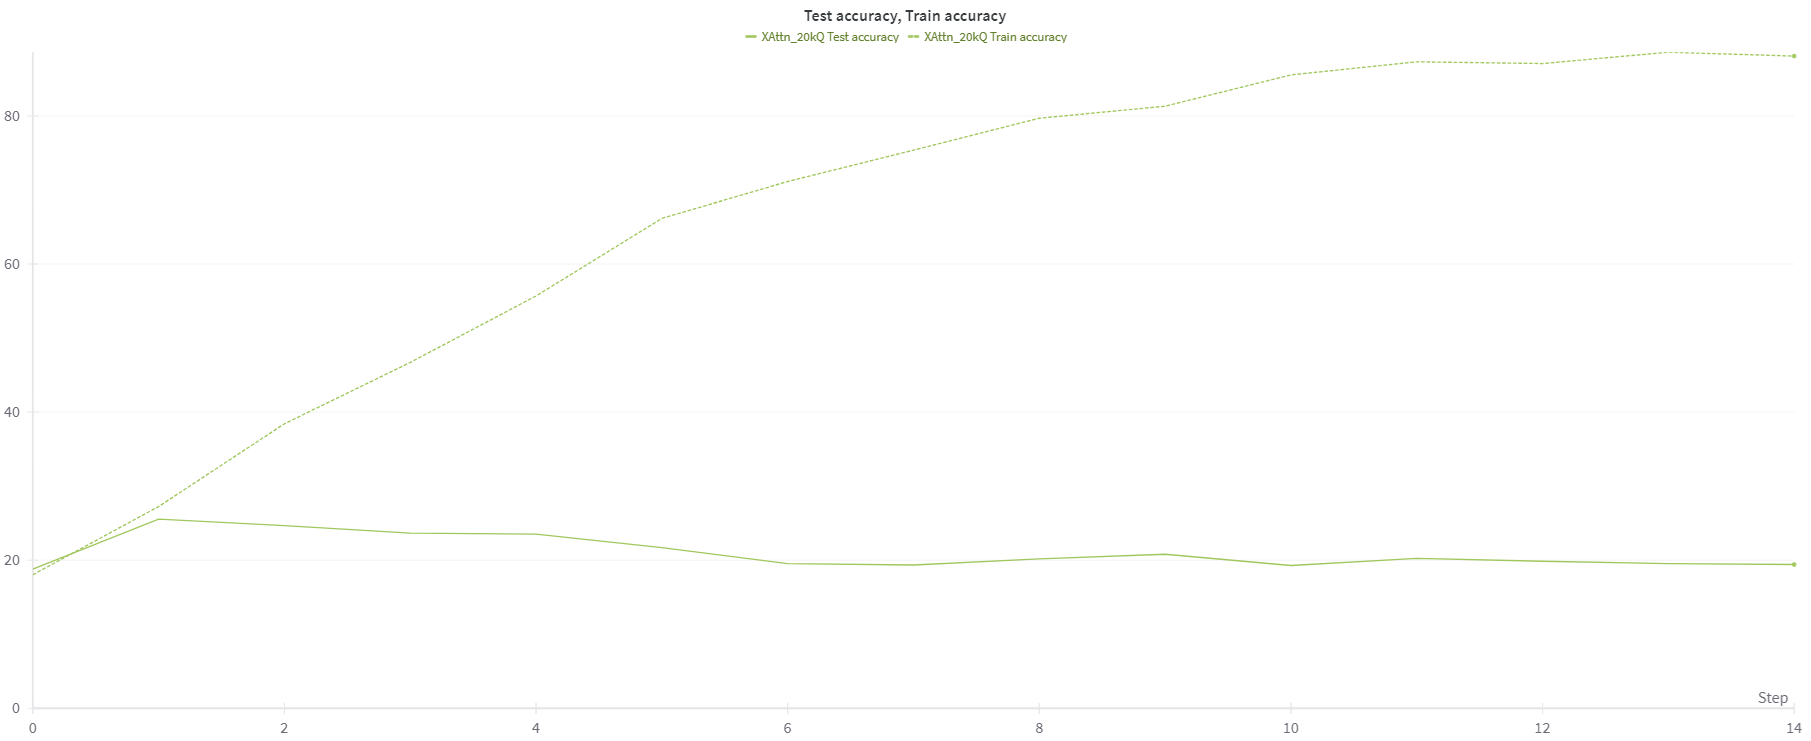
\includegraphics[width=0.4\textwidth]{images/acc.png}
%     \caption{}
%     \label{fig:example}
% \end{figure}
% \begin{figure}[h!]
%     \centering
%     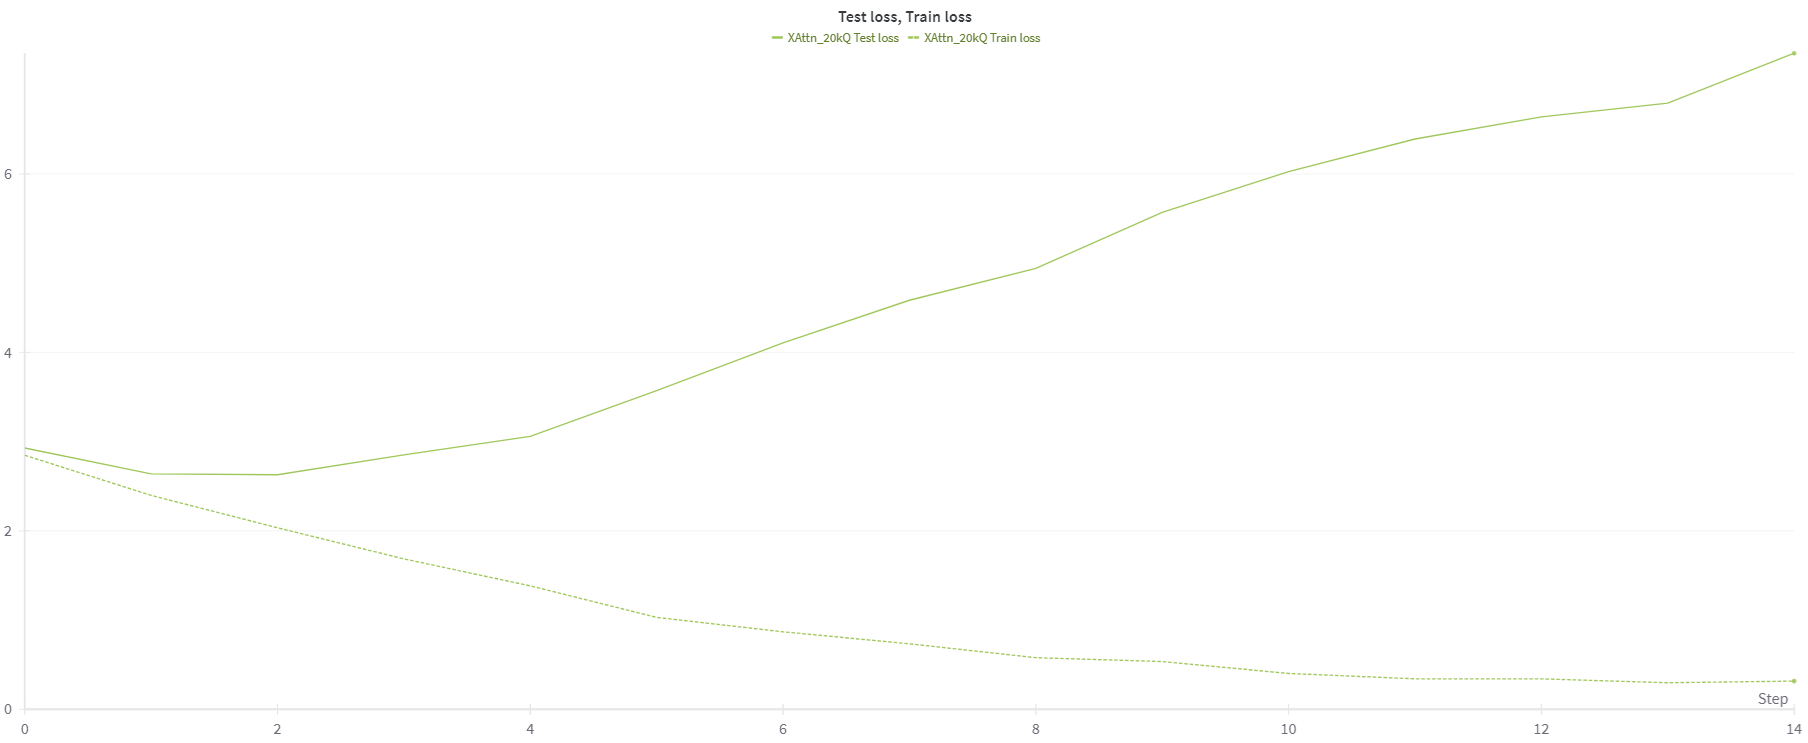
\includegraphics[width=0.4\textwidth]{images/loss.png}
%     \caption{}
%     \label{fig:example}
% \end{figure}


\subsubsection{Model Regularisation}
Overfitting is commonly caused by a model that is too complex, not regularized enough, not trained on enough data, or trained on poor quality data. To address this issue, we experiment with the following corrective approaches:
\begin{itemize}
    \item Weight decay (L2):
    \item Dropout:
    \item Increased batch size:
    \item Decreased LR:
    \item Normalization:
    \item Focal loss:
    \item Decreased model size: Number of parameters: Describe regular model (ScanSG-GNN) vs XS model (ScanSG-GNN-XS) vs. downsized model (ScanSG-GNN-32)
    \item Architectural changes: Removing some of the building blocks: Without GNN, without textencoder, with scene transformer encoder)
\end{itemize}

We retrain the ScanSG-GNN model with these changes on a smaller, $25\%$ of the dataset (5070 questions about 236 scenes). We evaluate the performance of each model with these changes on the test set of the ScanSG dataset, and report the best results in Table XXX.

\begin{table}[h!]
    \centering
    \caption{\textcolor{red}{redo these experiments if possible}}
    \begin{tabular}{l|c|}
    \cline{2-2}
                                              & \multicolumn{1}{l|}{\textbf{Test Accuracy}} \\ \hline
    \multicolumn{1}{|l|}{No changes}          & 20.1                                        \\ \hline
    \multicolumn{1}{|l|}{Batch size = 512}    & 17.9                                        \\ \hline
    \multicolumn{1}{|l|}{Weight decay = 1e-3} & 20.6                                        \\ \hline
    \multicolumn{1}{|l|}{LR = 1e-5}           & 17.5                                        \\ \hline
    \multicolumn{1}{|l|}{Normalization}       & 12.01                                       \\ \hline
    \multicolumn{1}{|l|}{Focal Loss}          & 19.0                                        \\ \hline
    \multicolumn{1}{|l|}{Dropout}             &                                             \\ \hline
    \multicolumn{1}{|l|}{XS model}            & 19.2                                        \\ \hline
    \end{tabular}
    \end{table}


We note that none of the regularization methods described above improved generalization. We therefore investigate the impact of data quality on the model's ability to generalize.

\subsection{Model Performance on Ideal Dataset}
We investigate the impact of the question dataset on model performance.
For these experiments, we split the ScanQA dataset into the following smaller datasets:

\begin{itemize}
    \item Easy dataset: contains only questions which contain the answer. Train set: 11806 questions about 555 scenes. Test set: 1083 questions about 71 scenes.
    \item Hard dataset: contains only questions which do not contain the answer. Train set: 7644 questions about 552 scenes. Test set: 498 questions about 71 scenes.
    \item Full dataset: contains all questions, same dataset as used in previous experiments.
\end{itemize}


\subsubsection{Ideal Graph Nodes, Full Question Dataset}
To understand the impact of the node embeddings on the model performance, we embed the object labels into graph nodes, rather than object images. The only difference from the previous experiment are the node embeddings. Table XX shows the results of this experiment.

\begin{table}[h!]
    \centering
    \caption{Performance on the full ScanSG+ScanQA dataset, with node embeddings computed from the object labels}
    \begin{tabular}{|l|c|l|l|l|}
    \hline
    \textbf{Model}         & \textbf{EM@1} & \textbf{EM@5} & \textbf{EM@10}  & \textbf{Sem-EM@1} \\ \hline
    Baseline               & 50.7 & 74.4 & 82.8 & 62.7 \\ \hline
    Baseline + GNN         & 16.2 & 45.3 & 62.1 & 24.7 \\ \hline
    ScanSG-GNN             & 33.1 & 73.1 & 88.0 & 43.6 \\ \hline
    ScanSG-noGNN           & \textbf{59.0} & \textbf{84.0} & \textbf{92.2} & \textbf{72.4} \\ \hline
    \end{tabular}
\end{table}

We note that results are significantly higher across all models, and the overfitting is slightly mitigated \textcolor{red}{add proof}. This shows that poor node embeddings contribute to overfitting, and low performance on the test set. The limitations of CLIP causing this were illustrated in Figure XX, and are further discussed in Section XX.
These results highlight the importance of high quality node embeddings.

The baseline outperforms the ScanSG-GNN model, and the ScanSG-noGNN is once more the best performing model.
To understand why this may be the case, we conduct the following experiments.

\subsubsection{Ideal Graph Nodes, Easy Question Dataset}

\begin{table}[h!]
    \centering
    \caption{\textcolor{red}{\textbf{Easy Q dataset Add semantic accuracy}}}
    \begin{tabular}{|l|c|l|l|l|}
    \hline
    \textbf{Model}         & \textbf{EM@1} & \textbf{EM@5} & \textbf{EM@10} & \textbf{Sem-EM@1} \\ \hline
    Baseline               & 67.3 & 91.7 & 96.6 & 83.3 \\ \hline
    Baseline + GNN         & 19.8 & 47.8 & 63.3 & 31.5 \\ \hline
    ScanSG-GNN             & 40.9 & 82.5 & 91.7 & 56.6 \\ \hline
    ScanSG-noGNN           & \textbf{76.0} & \textbf{93.6} & \textbf{97.1} & \textbf{95.0} \\ \hline
    \end{tabular}
\end{table}

results significantly higher and overfitting mitigated (show this somehow).
this method is likely better because we embed the exact label that appear in the question, so if the cross-attention mechanism works well, it just needs to select the word in the question which is also a node label.

\textcolor{red}{add attention pattern for not the best model here!! and show that the model just focuses on the matching word.}

+ and conclude that this model is good! (76) for easy input data!

\subsubsection{Ideal Graph Nodes, Hard Question Dataset}
\begin{table}[h!]
    \centering
    \caption{\textcolor{red}{\textbf{Easy Q dataset Add semantic accuracy}}}
    \begin{tabular}{|l|c|l|l|l|}
    \hline
    \textbf{Model}         & \textbf{EM@1} & \textbf{EM@5} & \textbf{EM@10} & \textbf{Sem-EM@1}\\ \hline
    ScanSG-GNN   & 24.7 & 57.6 & 72.3 & 29.7 \\ \hline
    ScanSG-noGNN & 34.9 & 62.4 & 77.9 & 43.0 \\ \hline
    \end{tabular}
\end{table}

If easy dataset is better with no-GNN because it doesnt need context awareness, maybe hard dataset can actually benefit from gnn module. so we test on hard data only and see if this is still true.

still true - 2 possible explanations for this:
- either the questions are just too hard and cant be answered (even i cant answer them tbh, there are too many possibilities)
- gnns are quite data hungry [reference] and there is not much "hard" data in this dataset. \textcolor{red}{to prove this, gradually increase datasize and show that adding more data slightly improves the proplem? maybe even do a projection of how many datapoints you would need?}

Also note that the gap between gnn and no-gnn is much smaller than in previous experiments.

todo: would be useful to take a look at which questions the gnn vs the no-gnn gets wrong.
%% ----------------------------------------------------------------------------
% CVG SA/MA thesis template
%
% Created 03/08/2024 by Tobias Fischer
%% ----------------------------------------------------------------------------
\newpage
\chapter{Discussion}
The discussion section gives an interpretation of what you have done \cite{day2006wap}:

\begin{itemize}
 \item \textit{What do your results mean?} Here you discuss, but you do not recapitulate results. Describe principles, relationships and generalizations shown. Also, mention inconsistencies or exceptions you found.
 \item \textit{How do your results relate to other's work?} Show how your work agrees or disagrees with other's work. You can rely on the information you presented in the ``related work'' section.
 \item \textit{What are the implications and applications of your work?} State how your methods may be applied and what implications might be. 
\end{itemize}

\noindent Make sure that the introduction/related work and the discussion section act as a pair, i.e. ``be sure the discussion section answers what the introduction section asked'' \cite{day2006wap}.

\begin{table}[h!]
    \centering
    \caption{\textcolor{red}{compare with original scanqa paper}}
    \begin{tabular}{|c|c|l|}
    \hline
    \textbf{Model}    & \textbf{EM@1} & \textbf{BLEU-1} \\ \hline
    ScanQA {[}...{]}  &  23.45        &  31.56          \\ \hline
    ScanQA2 {[}...{]} &  23.92        &  32.72          \\ \hline
    \end{tabular}
    \end{table}

\textbf{Are other methods doing this actually generalizing? Or are they just memorizing the dataset?} I don't really think our model is worse off than the others, i think all models suffer from the overfitting problem.

\textbf{Dataset size:} The dataset is relatively small, which might have an impact on the performance of the model - might not be able to generalize well to unseen data, overfitting to the training. 
For reference/comparison, the VQAv2 dataset has 1.1M questions, and the GQA dataset has 22M questions (2D VQA datasets). Yet we only have 20K

\textbf{Dataset quality:}
Dataset contents: most quesitons can be answered with 2d information only...

\textbf{Limitations of CLIP}
CLIP limitations (eg. high dimensional data, etc.)

\textbf{Requirements for a better dataset}

A lot of the other papers dont prove that the method is generalisable -- they do not report scores on other datasets and do not report the differnce in train/test accuracy. the only papers that do this are simple clip method.

\textbf{Future work}
could consider another way to encode the scene -- maybe add some kind of context nodes?

difficult to actually assess how integrating edge/context information is helpful for the VQA problem because we dont have a high quality question dataset. this should be a priori
%% ----------------------------------------------------------------------------
% CVG SA/MA thesis template
%
% Created 03/08/2024 by Tobias Fischer
%% ----------------------------------------------------------------------------

\chapter{Conclusion}

List the conclusions of your work and give evidence for these. Often, the discussion and the conclusion sections are fused. 




%% ----------------------------------------------------------------------------
% If Appendix is needed
%% ----------------------------------------------------------------------------
\appendix
%% ----------------------------------------------------------------------------
% CVG SA/MA thesis template
%
% Created 03/08/2024 by Tobias Fischer
%% ----------------------------------------------------------------------------
\chapter{The First Appendix}

In the appendix, list the following material: 

\begin{itemize}
 \item Data (evaluation tables, graphs etc.)
 \item Program code
 \item Further material 
\end{itemize}


%% ----------------------------------------------------------------------------
% Bibliography is stored in references.bib file, and can often be found
% online on webpages like dblp.uni-trier.de and Google Scholar
%
% To include it in your thesis, run
%  pdflatex main
%  bibtex main
%  pdflatex main
%  pdflatex main
%
% This ensures all references are done correctly.
%% ----------------------------------------------------------------------------

\bibliographystyle{plain}
\bibliography{references}

\end{document}

